\chapter{Dataset}
\label{ch:Dataset}

This chapter explains how the dataset is structured.

\section{Origin and Structure}
\label{sec:Origin and Structure}

The raman spectra in the dataset have been stored in a \textit{.parquet} file, which is a column-based format designed for efficient data storage and retrieval.

The analyzed biological tissue was taken from 25 different \textit{samples}, each one from a different patient.
From each sample, 1 to 5 areas called \textit{maps}, were then selected for the Raman spectra acquisition.
A spectrum was acquired for each pixel in the map, which has a size of 120x120 pixels.
Finally, each spectrum ranged across 483 bands, equivalent to wavenumbers (Raman shift).
Each spectrum (i.e. pixel) has an associated \textit{label}, indicating the type of biological tissue it belongs to.

\begin{table}[ht]
    \centering
    \begin{tabularx}{\textwidth}{|l|l|X|}
        \hline
        \textbf{Column} & \textbf{Format / Range} & \textbf{Description} \\
        \hline
        \texttt{Sample\_ID} & e.g. \texttt{1234\_567} & The first 4 digits identify the patient, the
                              last 3 the sample from that patient. \\
        \hline
        \texttt{Map\_ID}    & e.g. \texttt{Map\_1} & Acquisition map; 1 to 5 maps were
                              analysed per sample. \\
        \hline
        \texttt{x} & $x\in [0, 119]$ & Pixel coordinates on the horizontal axis\\
         \hline
        \texttt{y} & $y\in [0, 119]$ & Pixel coordinates on the vertical axis\\
        \hline
        \texttt{band\_}$n$  & $n \in [0, 482]$ & Raman intensity at the $n$-th spectral band,
                              for the 483 Raman shifts (cm$^{-1}$). \\
        \hline
        \texttt{Label}      & integer & Tissue-class identifier of the pixel (see Sec.~\ref{...}). \\
        \hline
    \end{tabularx}
    \caption{Structure of the dataset columns.}
    \label{tab:dataset-structure}
\end{table}

With 25 samples and 1 to 5 maps for each, the total number of maps is 78, thus amounting to 1\,123\,200 spectra.

\begin{figure}[ht]
    \centering
    
\includegraphics[width=0.5\linewidth]{Images/logo_polimi_scritta.eps}
    \caption{Relation between Sample, maps and spectra}
    \label{fig:placeholder}
\end{figure}



\section{Labels}
\label{sec:Labels}

\subsection{Histopathologist's classification}

Each pixel (spectrum) has been assigned a label, corresponding to a specific type of biological tissue, by a pathologist.
The classification pipeline started with the preparation of the samples as $12\mu m$ slices of tumoral tissue.
Raman spectroscopy was then performed on a slice, while the contiguous slice was treated with H\&E staining.
Classification was then performed on the stained slice by the histopathologist.
Finally the classification was applied to the Raman image.


This process includes multiple critical points:

\begin{itemize}
    \item Differences in composition for contiguous slices, leading to incorrect classification
    \item Human classification is not pixel-wise, as is artificial classification. Errors will be particularly common in boundaries between tissues
    \item Human misclassification of entire areas.
\end{itemize}

The provided labels have however been considered correct, as no other mean of comparison are available in current conditions.


\subsection{Labels analysis}[ht]
Biological tissues were divided in 14 classes, the most represented of which was the \textit{tumor} class. Occurrences for each class are shown in Fig.\ref{fig:label_distribution}
\begin{figure}
    \centering
    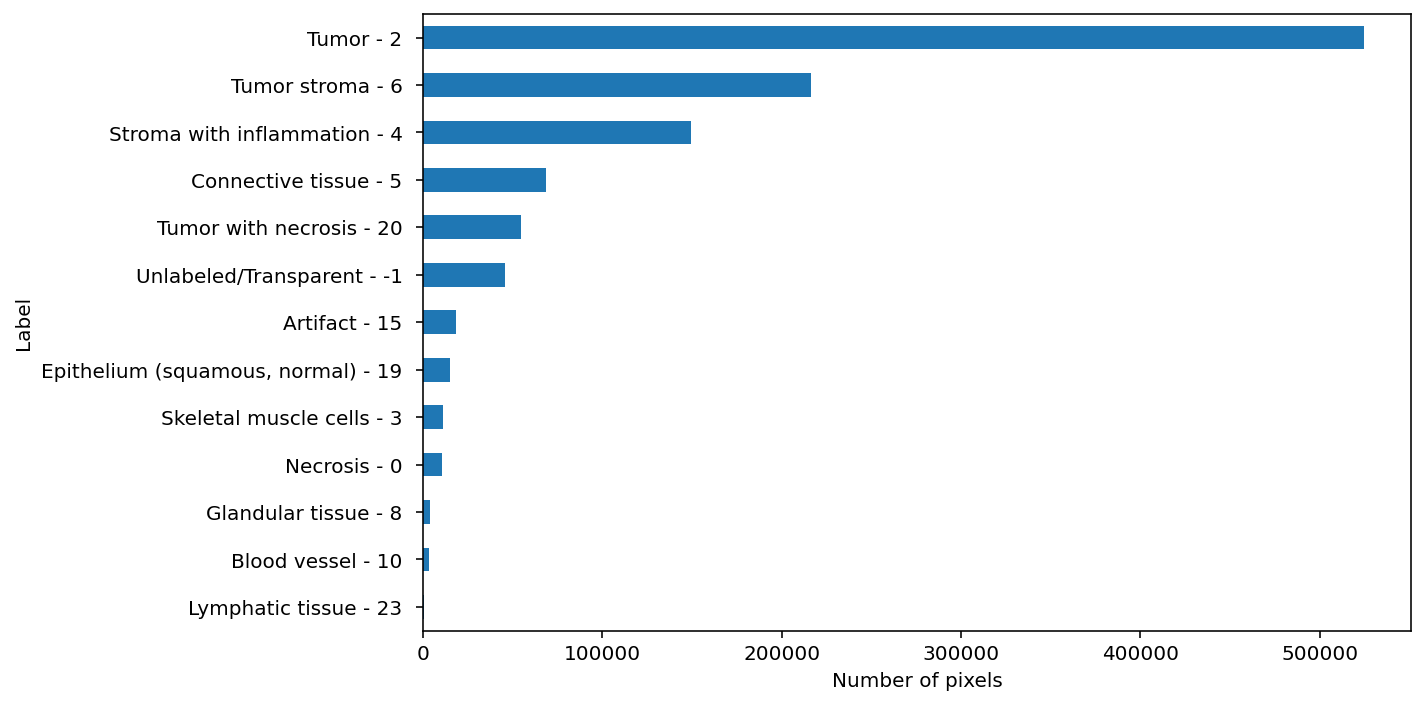
\includegraphics[width=0.75\linewidth]{Images/Images_ch_2/label_distributions.png}
    \caption{Occurrences for each label in the dataset}
    \label{fig:label_distribution}
\end{figure}

Elimination non relevant spectra for the dataset (i.e. unlabeled/transparent and artifacts) and binary grouping in tumoral/healty balances out the dataset (Fig.\ref{fig:binary_label_distribution})

\begin{figure}[ht]
    \centering
    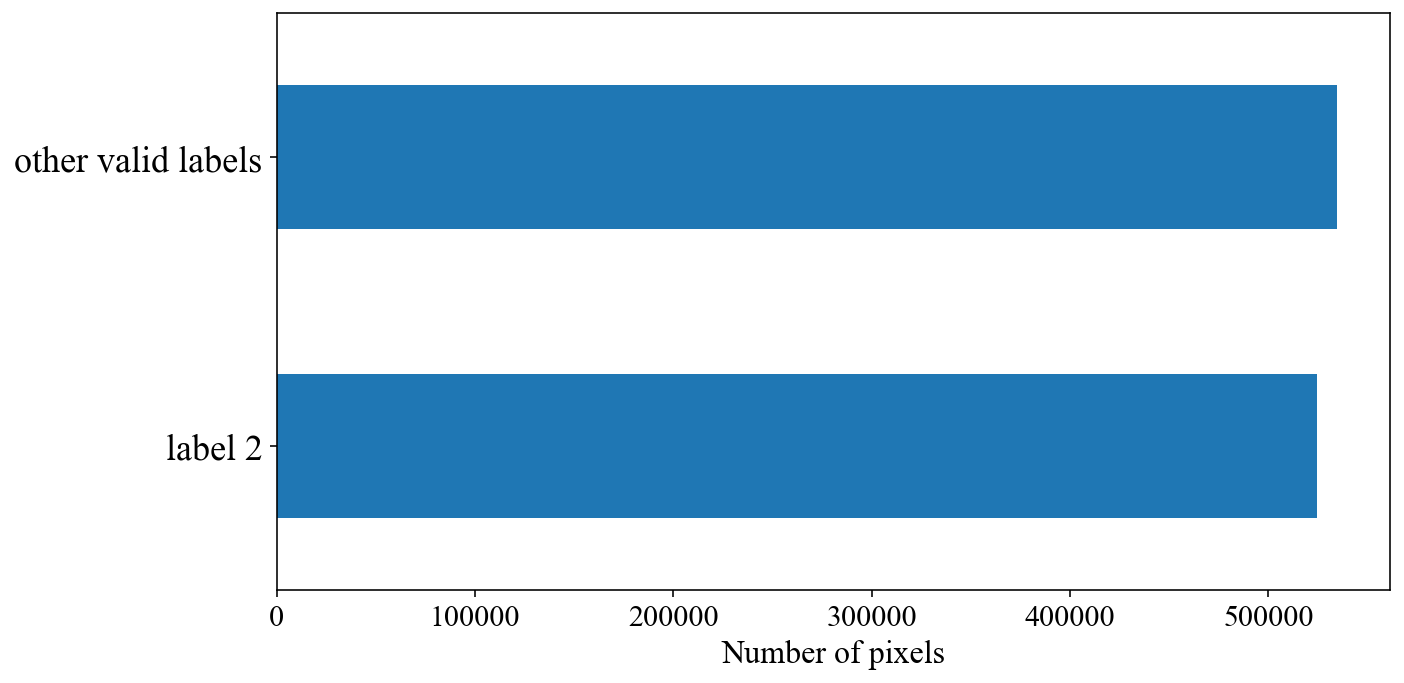
\includegraphics[width=0.75\linewidth]{Images//Images_ch_2/binary_label_distribution.png}
    \caption{Binary grouping by tumoral and healthy spectra after discarding unlabeled, transparent pixels and artifacts}
    \label{fig:binary_label_distribution}
\end{figure}

\section{Spectra}
\label{sec:Spectra}


\section{Binary classification}
\label{sec:Binary classification}